\subsection{How to draw the robot}
\frame
{
  \frametitle{How to draw the robot}
  
  \emph{An exocentric vision system for \textit{3m.o.r.d.u.c.} 
    needs to tell \textit{R.E.A.R.} how to draw the robot itself,
    by subclassing \textbf{Robot} class.}
  \pause

  \vskip15pt

  \begin{block} {\alert{\texttt{Concrete classes}}}

    \pause
    \begin{itemize}
      
    \item \alert{\textit{Morduc}} \\
      3m.o.r.d.u.c. 3D model in \textit{OpenGL}
      \visible<3>{
        \begin{center}
          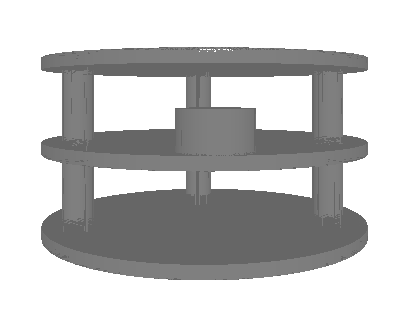
\includegraphics[width=80pt]{img/3morduc_opengl.png}
        \end{center}
      }
    \end{itemize}

  \end{block}
}

\subsection{How to choose the proper egocentric image}
\frame
{
  \frametitle{How to choose the proper egocentric image}
  
  \emph{An exocentric vision system for \textit{3m.o.r.d.u.c.} 
    needs to tell \textit{R.E.A.R.} how to choose the proper egocentric image,
    by implementig the \textbf{IImageSelector} interface.}
  \pause

  \vskip15pt

  \begin{block} {\alert{\texttt{Concrete classes}}}

    \begin{itemize}
      
    \pause
    \item \alert{\textit{SpacialMetricCalc}}
    \pause
    \item \alert{\textit{SweepMetricCalc}} \\
      details in next slide
    \pause
    \item \alert{\textit{AnotherSweepMetricCalc}} \\
      improvements of previous one, in order to
      provide user with more confortable teleguiding
      in case of strict turns

    \end{itemize}

  \end{block}
}

\subsubsection{Sweep Metric Algorithm}
\frame
{
  \frametitle{Sweep Metric Algorithm}
  
  \emph{Algorithm to choose the proper \textit{exocentric} image,
    among those collected.}
  \pause

  \begin{block} {\alert{\texttt{How it works}}}
 

    \begin{columns}
      
      \column{0.7\textwidth} {   
        \visible<2->{
          \begin{center}
            \only<2>{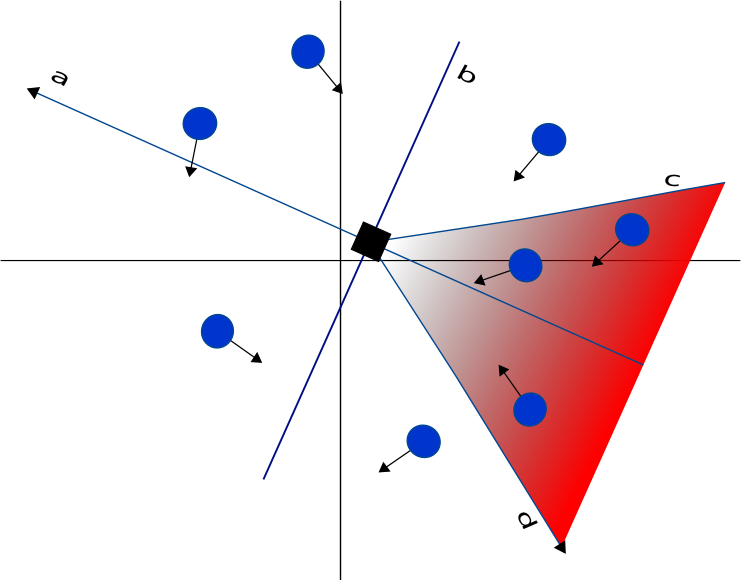
\includegraphics[width=0.8\textwidth]{img/sma_1.png}}
            \only<3>{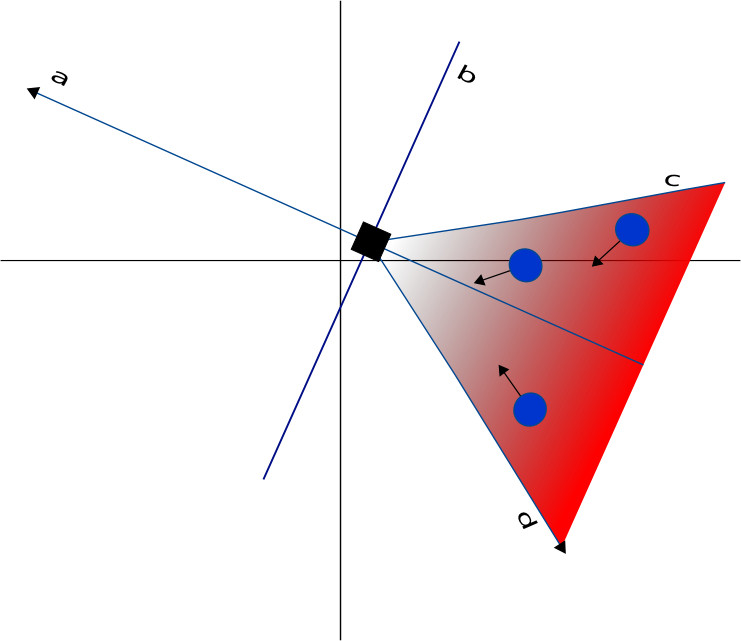
\includegraphics[width=0.8\textwidth]{img/sma_2.png}}
            \only<4>{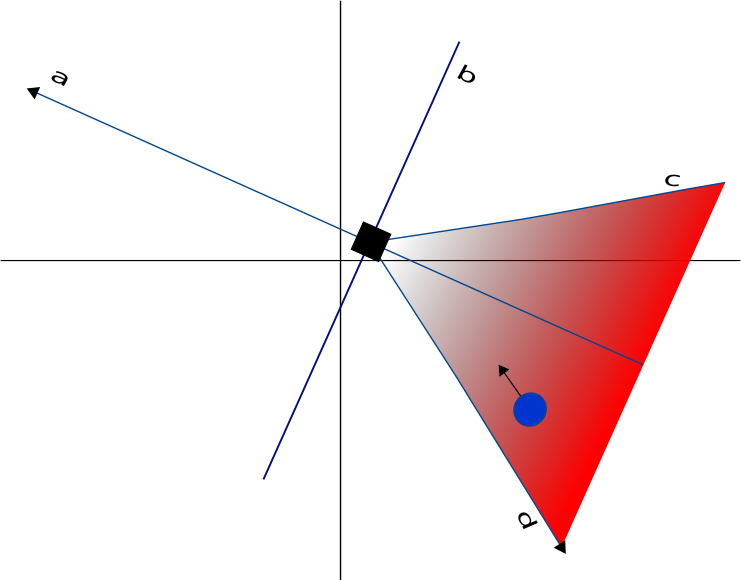
\includegraphics[width=0.8\textwidth]{img/sma_3.png}}
          \end{center}
        }
      }
      
      \column{0.2\textwidth} {
        \visible<2->{
          
          \scriptsize{Robot and image shot on XY plane}
          \vskip5pt
          
\includegraphics[width=8pt]{img/robot_icon.png} \\ 
          \tiny{robot oriented along sense indicated by line \textit{a}}
          \vskip5pt
          
\includegraphics[width=10pt]{img/image_icon.png} \\
          \tiny{image oriented along direction indicated by its arrow}
          \vskip5pt
          \tiny{red area indicates the \alert{\textit{sweep area}}}

        }
      }
      
    \end{columns}

    \vskip8pt
    
    \footnotesize{
      \only<2> {\alert{Step 0}: information about current robot position and image set are
      available.}
      \only<3> {\alert{Step 1}: discard all image shot outside the \textit{sweep area}.}
      \only<4> {\alert{Step 2}: discard all image shot with an orientation that differ more
        than a threadshold value from robot's orientation.}
     
    }
  \end{block}
}

\frame
{
  \frametitle{Sweep Metric Algorithm}
  
  \emph{Algorithm to choose the proper \textit{exocentric} image,
    among those collected.}

  \begin{block} {\alert{\texttt{How it works}}}
 
    At the end, three possible cases:
    \pause
    \begin{itemize}
      
    \item \alert{\textit{no images in \textit{sweep area}}} \\
      the egocentric image will be chosen
      \pause
      
    \item \alert{\textit{one image in \textit{sweep area}}} \\
      the unique image will be selected for exocentric vision
      \pause
      
    \item \alert{\textit{more than one image in \textit{sweep area}}} \\
      the image closer to an \textit{optimal distance} from the robot
      and with an orientation similar to robot's direction is chosen

      
    \end{itemize}
    
  \end{block}
}




\subsection{How to send and retrieve data to/from robot}
\frame
{
  \frametitle{How to send and retrieve data to/from robot}
  
  \emph{An exocentric vision system for \textit{3m.o.r.d.u.c.} 
    needs to tell \textit{R.E.A.R.} how to send and retrieve data to/from robot,
    by implementig the \textbf{IDataLogic} interface.}
  \pause

  \begin{block} {\alert{\texttt{Concrete classes}}}

    \begin{itemize}
      
    \pause
    \item \alert{\textit{DataLogicLogSimulator}} \\
      \footnotesize{
        new data are retrieved from log file written through
        a simulator session; acting
        in \textit{off-line} mode.
        }
    \pause
    \item \alert{\textit{DataLogicLogMorduc}} \\
      \footnotesize{
        new data are retrieved from log file written through
        a previous on-line teleguiding run accomplished with
        \textit{3m.o.r.d.u.c.}; acting
        in \textit{off-line} mode.
      }
    \pause
    \item \alert{\textit{DataLogicMorduc}} \\
      \footnotesize{
        new data and teleoperator's command are trasmitted from/to real 
        \textit{3m.o.r.d.u.c.}, through HTTP protocol; acting in
        \textit{on-line} mode.
      }
    \end{itemize}

  \end{block}
}


\subsection{Exocentric vs egocentric point of view}
\frame
{
  \frametitle{Exocentric vs egocentric point of view}
  
  \emph{Comparison between teleguiding \textit{3m.o.r.d.u.c.}
    form an egocentric and an exocentric point of view
    \footnote{\tiny{session recorded at DIIES laboratory}}.}
  \pause

  \begin{block} {\alert{\texttt{Teleoperator control}}}

    \begin{columns}
      
      \column{0.5\textwidth} {   
        \visible<2->{
          \footnotesize{Egocentric POV:}
          \begin{center}
            \only<2>{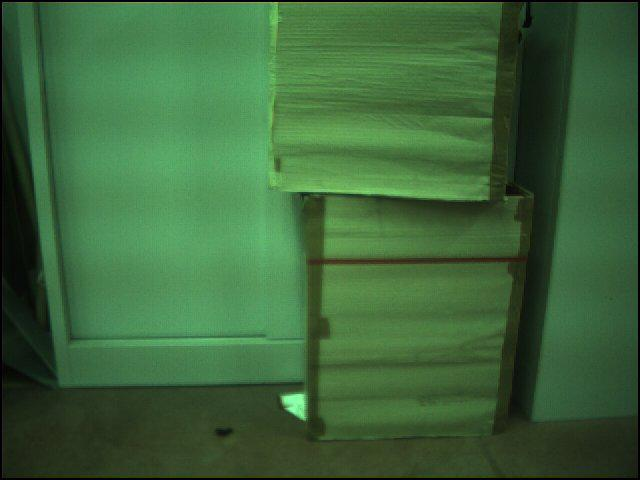
\includegraphics[width=0.9\textwidth]{img/log/img1.jpg}}
            \only<3>{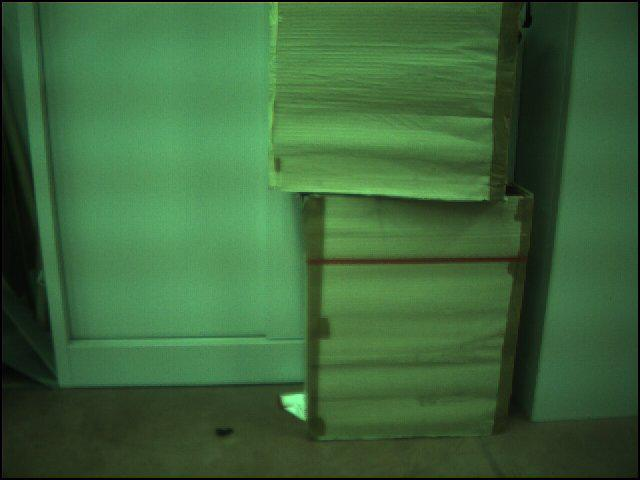
\includegraphics[width=0.9\textwidth]{img/log/img2.jpg}}
            \only<4>{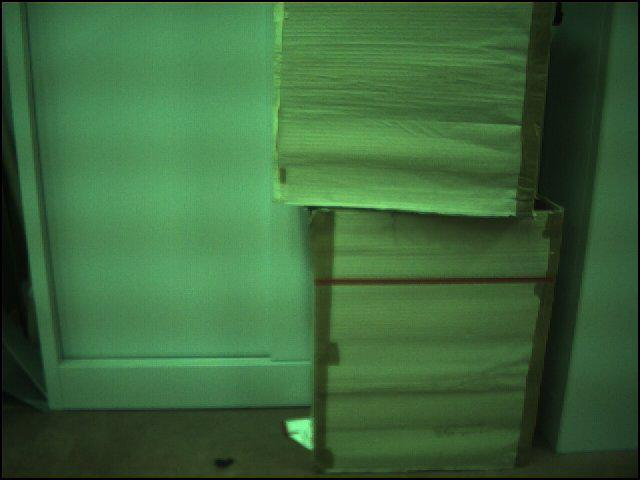
\includegraphics[width=0.9\textwidth]{img/log/img3.jpg}}
            \only<5>{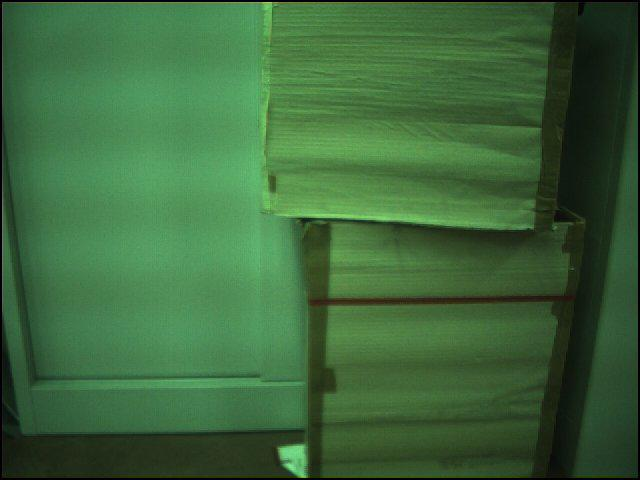
\includegraphics[width=0.9\textwidth]{img/log/img4.jpg}}
          \end{center}
        }
      }

      \column{0.5\textwidth} {   
        \visible<2->{
          \footnotesize{Exocentric POV:}
          \begin{center}
            \only<2>{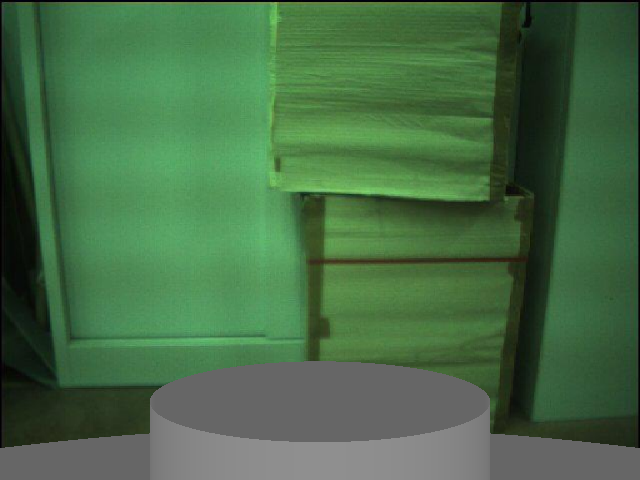
\includegraphics[width=0.9\textwidth]{img/screenshot/img1.png}}
            \only<3>{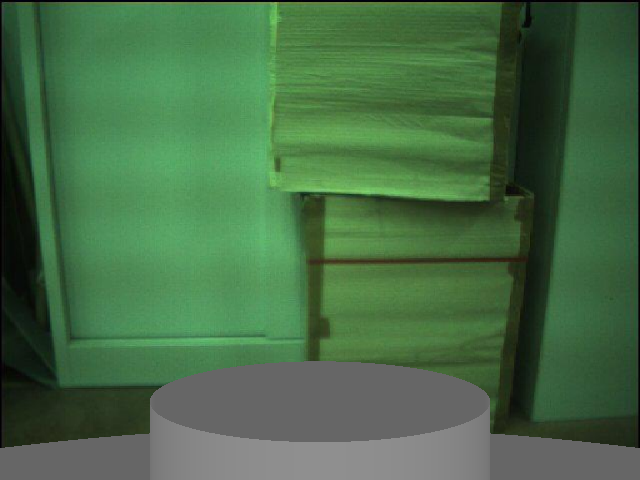
\includegraphics[width=0.9\textwidth]{img/screenshot/img2.png}}
            \only<4>{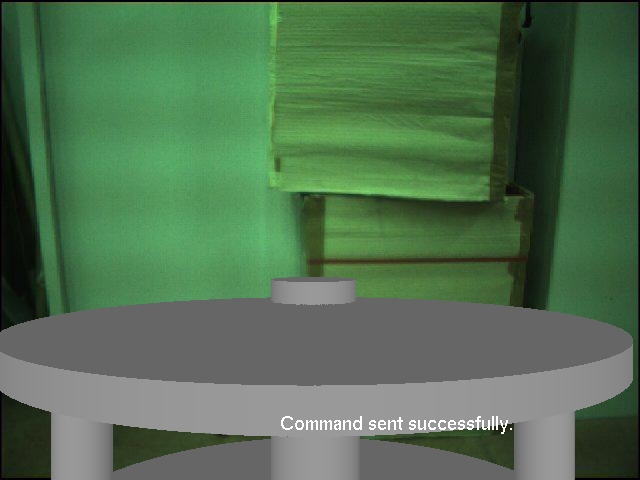
\includegraphics[width=0.9\textwidth]{img/screenshot/img3.png}}
            \only<5>{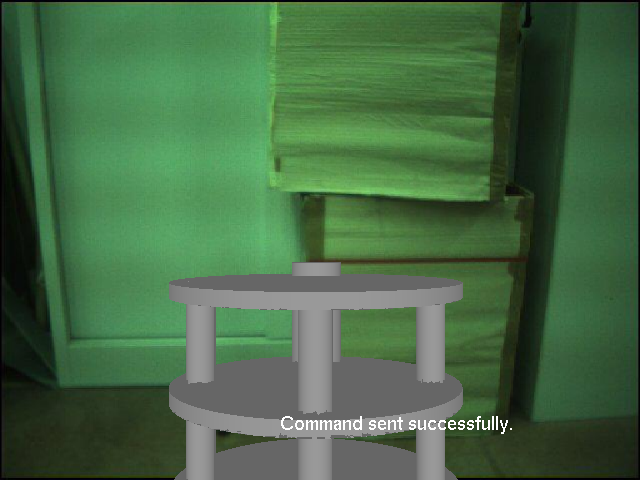
\includegraphics[width=0.9\textwidth]{img/screenshot/img4.png}}
          \end{center}
        }
      }

    \end{columns}

    \vskip20pt
    
    \only<2>{Next command: \alert{go forward}}
    \only<3>{Next command: \alert{go forward}}
    \only<4>{Next command: \alert{go forward}}
    \only<5>{Next command: \alert{go forward}}

  \end{block}
}
